% Drawing 154/06-10 -- folder 154, batch 06, archive page 112 (PDF page 113).
% Transcription: à droite, deux dessins en couleur : un croisement de droites orange enjambé par une courbe vert foncé, au-dessus d'une droite vert clair et de tirets, avec une flèche verticale ; puis la même configuration où la droite vert foncé passe par le croisement
% Kind: crossing straddled by a dark green curve; the same with the line through the crossing. Method 2 (schematic redraw from the facsimile). Status: ok.
% Notes: Right, two colour drawings: a crossing of orange lines straddled by a dark green curve (and its dashed double) above a light green line and dashes, with a vertical arrow; then the same configuration where the dark green line passes through the crossing, pencil hatching under it. Read from the page view.
% Coordinates: 1 unit = 1 mm = 1/100 of the crop width (bbox in page fractions: [0.705, 0.098, 0.9, 0.326]).
% Redrawn by Claude (claude-opus-5-5), issue #73, 2026-11-07; not checked by a human; not compiled (no TeX in the session).
% Rights: reproduces part of the work -- behind RENDER_TRANSCRIPTS, never published by itself.
\documentclass[tikz,border=3pt]{standalone}
\usepackage{amsmath,amssymb}
\usetikzlibrary{patterns,arrows.meta}
\tikzset{Or/.style={orange!90!black}, Ye/.style={yellow!80!orange}, Lg/.style={green!60!black!70}, Dg/.style={green!45!black}, Br/.style={brown!80!black}, Rd/.style={red!85!black}, Bl/.style={blue!70!black}, Gy/.style={black!40}, pencil/.style={black!45}, struck/.style={black!35}, mark/.style={circle,draw,inner sep=1.3pt}, pt/.style={circle,fill,inner sep=0.9pt}, opt/.style={circle,draw,fill=white,inner sep=1.1pt}}
\begin{document}
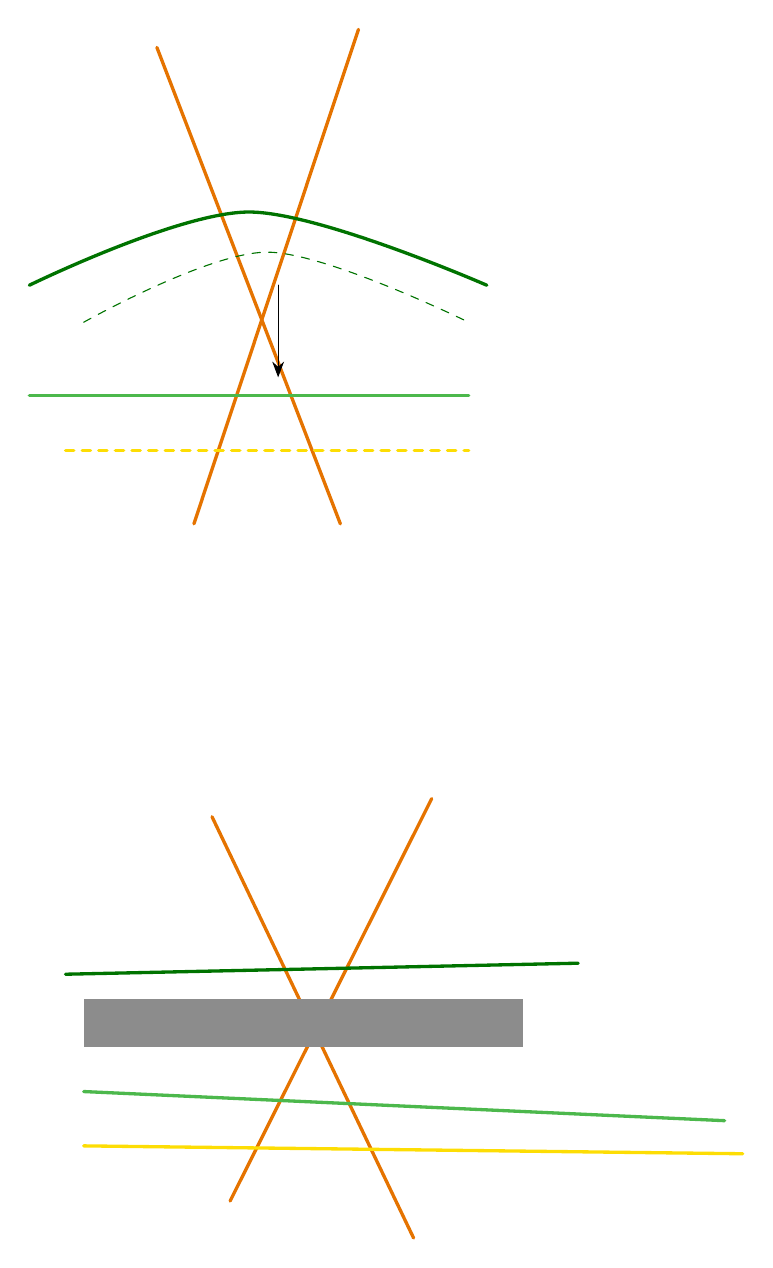
\begin{tikzpicture}[x=1mm,y=1mm,line cap=round,line join=round,font=\scriptsize]
\draw[Or,very thick] (20.9,-9.3) -- (44.2,-69.8);
\draw[Or,very thick] (46.5,-7) -- (25.6,-69.8);
\draw[Dg,very thick] plot[smooth, tension=0.55] coordinates {(4.7,-39.5) (32.6,-30.2) (62.8,-39.5)};
\draw[Dg,dashed] plot[smooth, tension=0.55] coordinates {(11.6,-44.2) (34.9,-35.3) (60.5,-44.2)};
\draw[Lg,very thick] (4.7,-53.5) -- (60.5,-53.5);
\draw[Ye,dashed,very thick] (9.3,-60.5) -- (60.5,-60.5);
\draw[-{Stealth[length=2mm]}] (36.3,-39.5) -- (36.3,-51.2);
\draw[Or,very thick] (30.2,-155.8) -- (55.8,-104.7);
\draw[Or,very thick] (27.9,-107) -- (53.5,-160.5);
\draw[Dg,very thick] (9.3,-127) -- (74.4,-125.6);
\fill[pattern=north east lines,pencil] (11.6,-130.2) -- (67.4,-130.2) -- (67.4,-136.3) -- (11.6,-136.3) -- cycle;
\draw[Lg,very thick] (11.6,-141.9) -- (93,-145.6);
\draw[Ye,very thick] (11.6,-148.8) -- (95.3,-149.8);
\end{tikzpicture}
\end{document}
